\documentclass[
    a4paper,
    12pt,
    fleqn,
    twoside
]{report}
\usepackage{duarte}
\usepackage{blindtext}
% ----------------------------
\begin{document}

% ============================
% CAPA
\begin{titlepage}
    
\sffamily
\centering
{\Large\bfseries São Paulo State University}

{\Large School of Engineering of Ilha Solteira}

\vfill

{\LARGE\bfseries Machine Learning: Optimizing Smart Systems with Artificial Intelligence}

\vfill

\begin{tabular}{ll}
    Student:        & Gabriel D. Silva \\
    Professor:      & Douglas D. Bueno
\end{tabular}

\vfill

Research Report --- Iniciação Científica 

\vfill

UNESP \\
Ilha Solteira - SP \\
2023
\end{titlepage}


% \begin{titlepage}
%     \sffamily
%     \begin{center}
%      {\LARGE \bfseries SÃO PAULO STATE UNIVERSITY}
     
%      {\LARGE School of Engineering of Ilha Solteira}
     
%      \vfill
     
%      {\Huge \bfseries DEEP LEARNING: APPLICATIONS IN THE MECHANICAL ENGINEERING CONTEXT}
     
%      \vfill
     
%      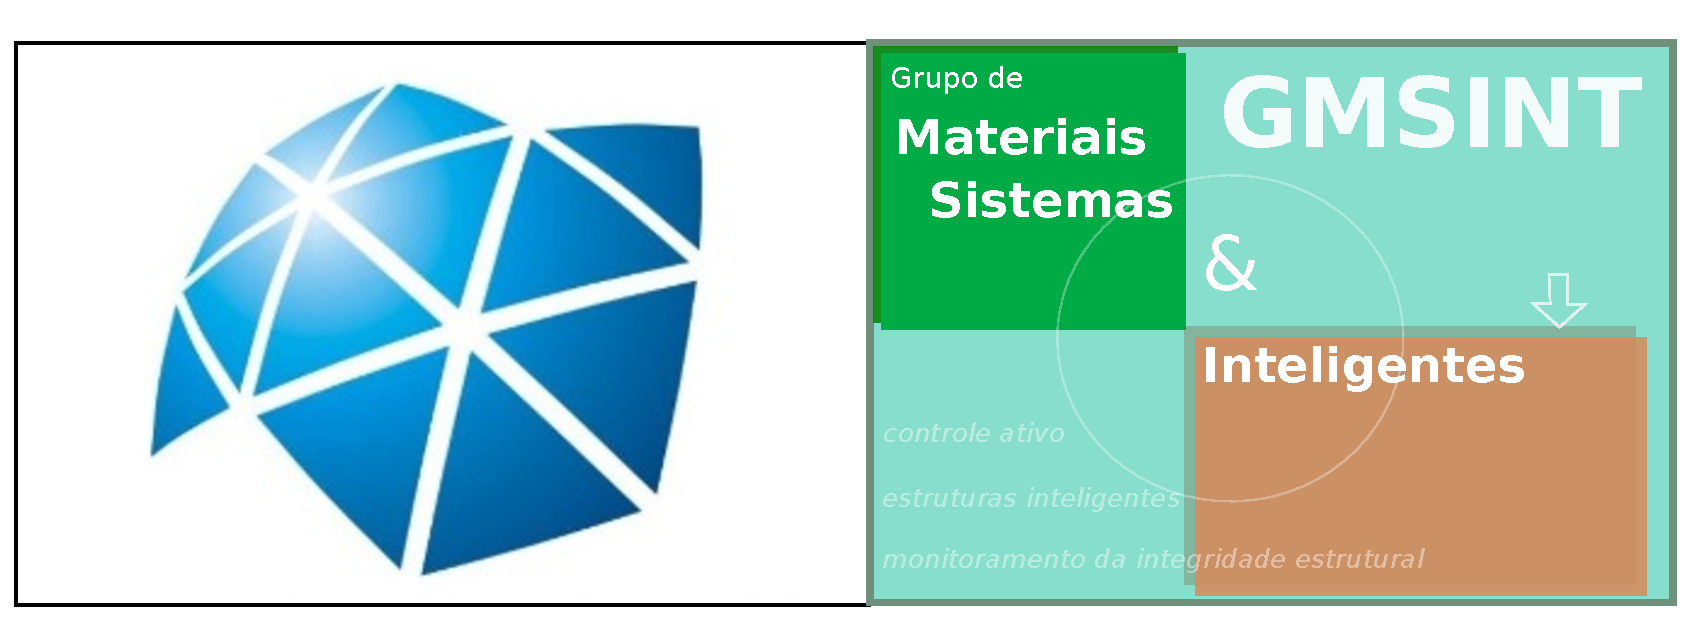
\includegraphics[width=\textwidth]{figures/logos/gmsint_logo.pdf}
     
%      \vfill
     
%      \begin{minipage}{0.7\textwidth}\centering
%       {\large \bfseries Research Report -- Iniciação Científica}
      
%       {\large \bfseries Student: Gabriel D. Silva}
      
%       {\large Professor: Douglas D. Bueno}
      
%      \end{minipage}
     
%      \vfill
     
%      {\large \bfseries UNESP}
     
%      {\large \bfseries Ilha Solteira -- SP}
     
%      {\large \bfseries 2023}
%     \end{center}
%    \end{titlepage}
% ----------------------------

% ============================
% RELATÓRIO DE PESQUISA
\setcounter{page}{1}
\pagenumbering{roman}
\pagestyle{empty}
\begin{center}
	\vspace{100pt}
	{\Large\scshape\bfseries Research Report}
\end{center}
\noindent
The present report approaches a way to improve smart systems. Through artificial intelligence applied in the mechanical engineering field, it provides a consistent algorithm that can reads data, trains the machine and provides results about the situation and what to do with it. It will be studied two cases, one of them using machine learning classical techniques to determine the forces applied to a unnamed aerial vehicle and other using deep learning techniques like neural networks in the structural health monitoring area. 

\noindent
\textcolor{red}{Complete after the research is done.}

\noindent
{\bfseries Keywords:} machine learning, structural health monitoring, unnamed aerial vehicle

\clearpage
% ----------------------------

% ============================
% LISTA DE FIGURAS
% {\sffamily\listoffigures}
% \newpage
% ----------------------------

% ============================
% LISTA DE TABELAS
% {\sffamily\listoftables}
% \newpage
% ----------------------------

% ============================
% LISTA DE ABREVIAÇÕES
% \printglossary
% \newpage
% ----------------------------

% ============================
% SUMÁRIO
{\sffamily\tableofcontents}
\newpage
% ----------------------------

% ============================
% FORMATAÇÕES EXTRAS
\setcounter{page}{1}
\pagenumbering{arabic}
\pagestyle{fancy}
% ----------------------------

% ============================
% SEÇÕES
\chapter{Literature Review}\label{sec:literature_review}

This chapter deals with the history, the main concepts and some practical cases of \gls*{shm} inside the industry and academic area, besides showing how it may be used in the railway crack detection context.
Next, in the dynamic field, it will be studied the main mechanical concepts to get the necessary understanding to an \gls*{uav} motion as well the basics to know how an \gls*{uav} can be controlled.
Then, it will be shown the mathematics behind the algorithms of deep learning that will be implemented in the \cref{sec:results}. 
Finally, the way how the algorithms are going to be implemented and the tools necessary to achieve the desired \gls*{nn}.

\input{sections/body/methodology/ai.tex}
% ----------------------------

% ============================
% REFERÊNCIAS
% \printbibliography
\bibliographystyle{chicago}
\bibliography{ref}
% ----------------------------

% ============================
% APÊNDICE
\appendix
\titleformat{\chapter}{\sffamily\centering\bfseries\large}%
{APPENDIX \thechapter \,--}{1mm}{\large}
\chapter{Codes}

% ============================
% RELATÓRIO DE PESQUISA
\end{document}